\section{Model Architectures}
\label{sec:architecture}

To address the facial emotion recognition task (FER), our group investigates multiple
convolutional neural networks (CNNs) that have demonstrated strong performance in image
classification and facial analysis tasks. CNNs build the base for most of our models. This 
decision is based on according literature emphasizing the clear performance advantage of 
CNNs compared to other approaches such as traditional machine learning models 
\cite{Dong_2024}. Each team member focuses on implementing and evaluating selected
architectures in order to identify the most suitable model for achieving a high 
classification accuracy while maintaining robust generalization performance.

\begin{itemize}
    \item Dmytro Dumanskyy: 
    \item Tiago Kienzle Hagen: ResNet, CERN, Poster++
    \item Aleksandar Neshov: ResNet, EfficientNet, DenseNet
    \item Daniel Pfefferkorn: GoogLeNet, VGG-19, EmoNeXt
\end{itemize}

Maximizing the accuracy of the FER task represents the core goal of our group. Apart 
from the aforementioned aspects, the actual architecture of our neural network plays 
a key role in achieving this goal to the best of our ability. In the follwoing section 
we want to highlight our decision making process.

\subsection{Criteria for model selection}

The suitability of a model for this project is evaluated based on the following 
criteria:

Firstly the design should be well documented in the literature to ensure scientifically 
proven effectiveness. For a model to be taken into closer consideration it should have 
reported strong results on standart benchmarks.

Secondly the architecture should be capable of extractig important  facial featrures 
such as the eyes, the eyebrows and the mouth meaningfully.

Finally models that are prone to overfitting are seen as unfavorable for our project. 
The chosen network should be able to learn distinctive features well while not overly 
relying on a high number of samples to achieve acceptable results. Since FER datasets 
are limited in sample size, we will prioritize models that shine through their data 
efficiency.

\begin{figure}[h]
    \centering
    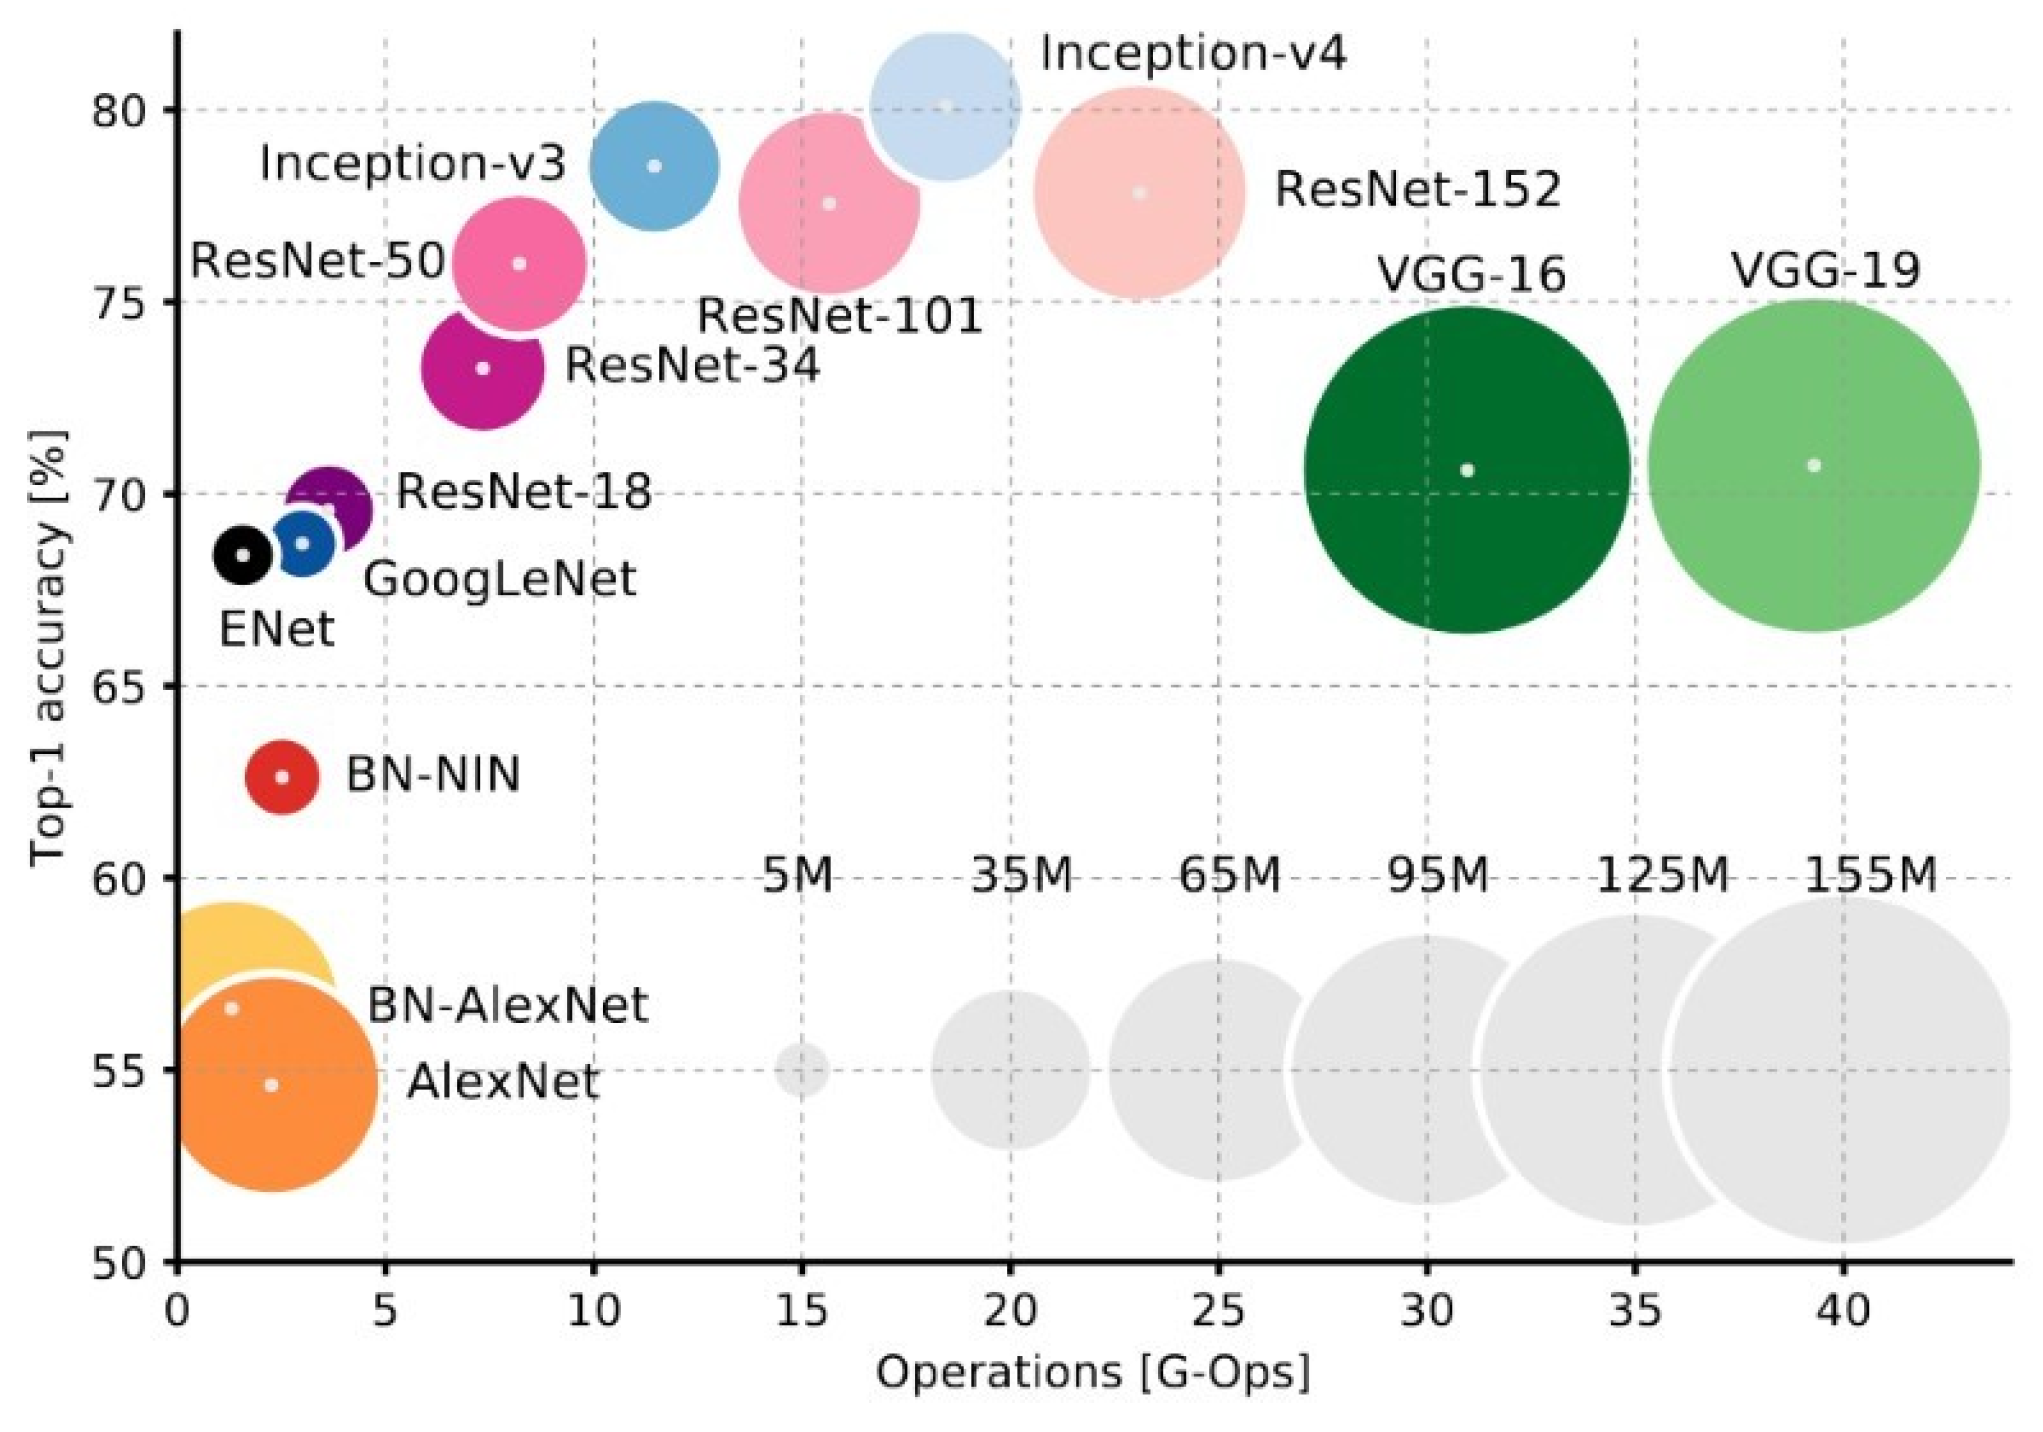
\includegraphics{figures/Model_Comparison.png}
    \caption{This figure from \citet{info15030135} was used as a general
    reference as to which models to take into consideration.}
    \label{fig:accuracies}
\end{figure}

\subsection{Excluded model architectures}

Not all types of models were categorized as suitable for the task at hand. Vision Transformers 
(ViT) are highly data hungry and tyically rely on large-scale pretraining, making them suboptimal
for training from scratch on limited FER datasets. Furthermore any outdated neural networks that 
are no longer competitive in terms of accuracy or efficiency were used as baselines for 
comparison.

\subsection{Training setup}

We decided to research common training parameters used in scientific papers that yielded good 
results. All models are trained from scratch using a consistent training protocol to ensure fair
comparison.

We decided to use Cross-Entropy loss as our loss function since it's widely used in similar 
classification tasks. Using Stochastic gradient descent (SGD) as our optimizer we are going to 
train the networks for approximately 30-50 epochs depending on individual model convergence.
Furthermore we plan on exploring attention mechanisms to improve robustness against facial 
occlusions.

To ensure a consistent baseline fo rmodel evaluation all models are trained and tested on a 
predefined dataset.

\subsection{Model selection strategy}

We are currently in theprocess of deciding on a final neural network design for the entire group.
Each team member is implementing their own model based on the architectures described above. The
final model will be decided through the highest test accuracy on our collective test set.
